\section{Actuators}\label{sec:Motor}
There are two actuators in the system, a brushless DC-motor as the main actuator which is used to apply the required control action and aservo motor, which can be used to brake the wheel in order to raise the frame.

\subsection{Brushless DC-Motor}
The brushless DC-motor is attached to the wheel and it is in charge of providing the required torque to the system.
It is an EC 45 flat 50 Watt (part no. 251601), which has additional features such three Hall effect sensors for angular velocity measurements.
%can take a nominal current of 2.33 A, and 23 A at very short peaks.It has a mechanical time constant of 12,4 ms \cite{MaxonMotors}. The nominal current puts a limit on the control signal that can be sent to the motor control board.\fxnote{Should this control signal be mentioned here?}.
%\fxnote{Should there be made a table listing the motors data instead of writing a paraghap with the info?}
Table~\ref{BrushlessDCMotorTable} contains some of the characteristics for this motor.

\begin{table}[H]
	\centering
	\begin{tabular}{|p{4.8cm}|p{3.3cm}|}
		\hline%------------------------------------------------------------------------------------
		\textbf{Motor Data}                        &  \textbf{Value} \unitWh{Unit}  \\
		\hline%------------------------------------------------------------------------------------
%		Max voltage                               &  24 \unitWh{V}  	\\
%		\hline%------------------------------------------------------------------------------------
		Nominal current                   		  &  2,33 \unitWh{A}	\\
		\hline%------------------------------------------------------------------------------------
		Motor constant (\si{K_t})				 &  33,5 \unitWh{N\cdot m \cdot A^{-1}}  \\
		\hline%------------------------------------------------------------------------------------
		Mechanical time constant                 &  12,4 \unitWh{ms}  \\
		\hline%------------------------------------------------------------------------------------
	\end{tabular}
	\caption{Important parameters of the brushless DC-motor}
	\label{BrushlessDCMotorTable}
\end{table}


\subsection{Motor Control Board}
There is a motor control board, Maxon ESCON Module 50/5, connected between the BeagleBone and the brushless DC-motor, and it is specifically made to work with ESCON motors.

The following table shows some of the main characteristics of the board.

\begin{table}[H]
	\centering
	\begin{tabular}{|p{7cm}|p{2.3cm}|}
		\hline%------------------------------------------------------------------------------------
		\textbf{Characteristics}                 &  \textbf{Value} \unitWh{Unit}  \\
		\hline%------------------------------------------------------------------------------------
		Nominal output current                   &  5 \unitWh{A}  	\\
		\hline%------------------------------------------------------------------------------------
		Peak current (<20 s)                     &  15 \unitWh{A}	\\
		\hline%------------------------------------------------------------------------------------
		Current control PWM frequency 				   &  53,6 \unitWh{kHz}  \\
		\hline%------------------------------------------------------------------------------------
		Sample Rate of PI current controller     &  53,6 \unitWh{kHz}  \\
		\hline%------------------------------------------------------------------------------------
	\end{tabular}
	\caption{Important parameters of the motor control board}
	\label{MotorControlBoardTable}
\end{table}
%The PWM signal has a range of 10 \% to 90 \%. 
%Inside the board is a 4-quadrant configuration.\\
The motor control board can be configured with a program provided by Maxon called ESCON studio.\cite{ESCONStudio}\\ 
The board is set to run with a closed loop control for the current. It is assumed that the reference current is the one given to the motor so the loop can be seen just as a unit gain. This assumption is validated through a test described in \appref{app:motorCurrentTest}, where it can be seen that both currents can be assumed to be equal.

\begin{figure}[H]
	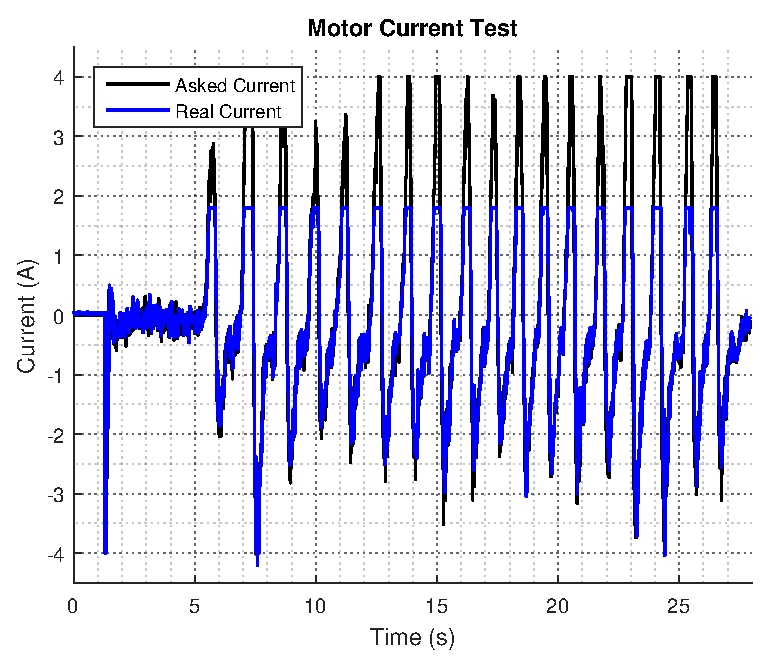
\includegraphics[scale=.75]{figures/motorCurrentTest}
	\centering
	\caption{Result of the test done to the motor to check that the reference current }
\end{figure} \label{motorCurrentTest2}

The reference current is sent to the control board as a PWM signal, whose duty cycle is configured within the range of 10 \% to 90 \% corresponding to \SI{4}{A} at 90 \% and \SI{-4}{A} at 10 \%. All the configurations can be seen \appref{MaxonControlESCON}.


\subsection{Braking System}
There is a braking mechanism included in the system, which can be used to make the frame go from resting position to vertical position.

To perform this task the brushless DC-motor spins up the reaction wheel and when it has enough kinetic energy the braking mechanism suddenly brake it, using for this task a Hitec HS225 Mighty Mini Servomotor. The inertia of the wheel is thus transfered to the frame, in order to raise it to standing position.

%The brake system is however not used in this project, since the jump up procedure is out of its scope.

%\fxnote{For gods sake fix this table!..:p}
%\begin{table}[H]
%	\centering
%	\begin{tabular}{|l|llll|}
%		\hline%------------------------------------------------------------------------------------
%		\textbf{Characteristics}           & \textbf{Values} &                      &  &\\
%		\hline%------------------------------------------------------------------------------------
%		Reaction time                      & @\SI{4,8}{V}    &\si{0,14/60} \si{s\cdot deg^{-1}} &and @\SI{6,0}{V} \si{0,11/60} &\si{s\cdot deg^{-1}} \\
%		\hline%------------------------------------------------------------------------------------
%		Speed                              & @\SI{4,8}{V}    &\SI{7,48}{rad\cdot s^{-1}} &and @\SI{6,0}{V} \si{9,52} &\si{rad\cdot s^{-1}}             \\
%		\hline%------------------------------------------------------------------------------------
%		Torque                             & @\SI{4,8}{V}    &\SI{3,9}{kgF\cdot cm} &and @\SI{6,0}{V} \si{4,8} &\si{kgF\cdot cm} \\
%		\hline%------------------------------------------------------------------------------------
%		Size                							 &  \multicolumn{4}{l|}{\si{32,26\ x\ 16,76\ x\ 31,00} \si{mm}}             \\
%		\hline%------------------------------------------------------------------------------------
%		Weight                             &  \SI{27,94}{g}  &                       &     &        \\
%		\hline%------------------------------------------------------------------------------------
%	\end{tabular}
%	\caption{Hitec HS225 Mighty Mini Servomotor Specifications}
%	\label{HitecHS225Servomotor}
%\end{table}